% 
% Annual Cognitive Science Conference
% Sample LaTeX Paper -- Proceedings Format
% 

% Original : Ashwin Ram (ashwin@cc.gatech.edu)       04/01/1994
% Modified : Johanna Moore (jmoore@cs.pitt.edu)      03/17/1995
% Modified : David Noelle (noelle@ucsd.edu)          03/15/1996
% Modified : Pat Langley (langley@cs.stanford.edu)   01/26/1997
% Latex2e corrections by Ramin Charles Nakisa        01/28/1997 
% Modified : Tina Eliassi-Rad (eliassi@cs.wisc.edu)  01/31/1998
% Modified : Trisha Yannuzzi (trisha@ircs.upenn.edu) 12/28/1999 (in process)
% Modified : Mary Ellen Foster (M.E.Foster@ed.ac.uk) 12/11/2000
% Modified : Ken Forbus                              01/23/2004
% Modified : Eli M. Silk (esilk@pitt.edu)            05/24/2005
% Modified: Niels Taatgen (taatgen@cmu.edu) 10/24/2006

%% Change ``a4paper'' in the following line to ``letterpaper'' if you are
%% producing a letter-format document.

\documentclass{article} % For LaTeX2e

\usepackage{nips12submit_e,times}
\usepackage{pslatex}
\usepackage{amsmath}
\usepackage{amsfonts}
\usepackage{latexsym}
\usepackage{amssymb}
%\usepackage{apacite}
\usepackage{graphicx}
\usepackage{xspace}
\usepackage{multirow}
\usepackage{array}
\usepackage{caption}
\usepackage{subcaption}
\usepackage[numbers]{natbib}

\newcommand{\dictionary}{\ensuremath{\mathcal{D}}\xspace}

\title{Halo, Hyperbole, and the Pragmatic \\ Interpretation of Numbers}
 
\author{
Jean Y. Wu \\
Symbolic Systems Program\\
Stanford University\\
Stanford, CA 94305 \\
\texttt{jeaneis@stanford.edu} \\
\And
Justine T. Kao \\
Department of Psychology\\
Stanford University \\
Stanford, CA 94305 \\
\texttt{justinek@stanford.edu} \\
\AND
Leon Bergen \\
Department of Brain and Cognitive Sciences\\
Massachusetts Institute of Technology \\
Cambridge, MA 02138\\
\texttt{bergen@mit.edu} \\
\And
Noah D. Goodman \\
Department of Psychology\\
Stanford University \\ 
Stanford, CA 94305\\
\texttt{ngoodman@stanford.edu} \\
}


\begin{document}
\title{Supplementary: \\ Halo, Hyperbole, and the Pragmatic \\ Interpretation of Numbers}
\maketitle

\section{Behavioral Experiment}

\subsection{Procedures}

\begin{table}[h]
\begin{tabular}{| p{0.15cm}  p{8.15cm}| p{0.15cm}p{4cm} |}\hline
\multicolumn{2}{|c|}{\textbf{Scenario}} & \multicolumn{2}{|c|}{\textbf{Values for X}} \\\hline
\multicolumn{2}{|l|}{Ann and Bob are friends. They are taking the same class.} & \multicolumn{2}{|l|}{[$100$, $102$, $150$, $152$,}\\
\multicolumn{2}{|l|}{\textbf{Ann:} ``How much did the textbook cost you?"} & \multicolumn{2}{|l|}{$200$, $202$, $1000$, $1012$]}\\
\multicolumn{2}{|l|}{\textbf{Bob:} ``\{X\} dollars."} & \multicolumn{2}{|l|}{}\\\hline
\multicolumn{2}{|c|}{\textbf{Questions}} & \multicolumn{2}{|c|}{\textbf{Responses}} \\\hline
(1) & Was Bob being literal about the cost of the textbook, & (1) &[Literal / Exaggerating] \\
 & or was he exaggerating? & (2) & [Free response] \\
(2) & How much do you think the textbook actually cost? & (3) & [Likert scale] \\
(3) & How negative does Bob feel about the cost of the textbook? & (4) & [Exactly \{X\} dollars / \\
(4) & What is Bob most likely trying to communicate by saying  ``\{X\} dollars"? & & Approximately \{X\} dollars/ The textbook is expensive and Bob is not happy.]\\\hline
\end{tabular}
\caption{Parking ticket costs scenario}
\label{tab:myfirsttable}
\end{table}

\begin{table}[h]
\begin{tabular}{| p{0.15cm}  p{8.15cm}| p{0.15cm}p{4cm} |}\hline
\multicolumn{2}{|c|}{\textbf{Scenario}} & \multicolumn{2}{|c|}{\textbf{Values for X}} \\\hline
\multicolumn{2}{|l|}{Ann and Bob are friends. They are taking the same class.} & \multicolumn{2}{|l|}{[$100$, $102$, $150$, $152$,}\\
\multicolumn{2}{|l|}{\textbf{Ann:} ``How much did the textbook cost you?"} & \multicolumn{2}{|l|}{$200$, $202$, $1000$, $1012$]}\\
\multicolumn{2}{|l|}{\textbf{Bob:} ``\{X\} dollars."} & \multicolumn{2}{|l|}{}\\\hline
\multicolumn{2}{|c|}{\textbf{Questions}} & \multicolumn{2}{|c|}{\textbf{Responses}} \\\hline
(1) & Was Bob being literal about the cost of the textbook, & (1) &[Literal / Exaggerating] \\
 & or was he exaggerating? & (2) & [Free response] \\
(2) & How much do you think the textbook actually cost? & (3) & [Likert scale] \\
(3) & How negative does Bob feel about the cost of the textbook? & (4) & [Exactly \{X\} dollars / \\
(4) & What is Bob most likely trying to communicate by saying  ``\{X\} dollars"? & & Approximately \{X\} dollars/ The textbook is expensive and Bob is not happy.]\\\hline
\end{tabular}
\caption{Example scenario of textbook costs}
\label{tab:myfirsttable}
\end{table}



\begin{table}[h]
\begin{tabular}{| p{0.15cm}  p{8.15cm}| p{0.15cm}p{4cm} |}\hline
\multicolumn{2}{|c|}{\textbf{Scenario}} & \multicolumn{2}{|c|}{\textbf{Values for X}} \\\hline
\multicolumn{2}{|l|}{Ann and Bob are friends. They are taking the same class.} & \multicolumn{2}{|l|}{[$100$, $102$, $150$, $152$,}\\
\multicolumn{2}{|l|}{\textbf{Ann:} ``How much did the textbook cost you?"} & \multicolumn{2}{|l|}{$200$, $202$, $1000$, $1012$]}\\
\multicolumn{2}{|l|}{\textbf{Bob:} ``\{X\} dollars."} & \multicolumn{2}{|l|}{}\\\hline
\multicolumn{2}{|c|}{\textbf{Questions}} & \multicolumn{2}{|c|}{\textbf{Responses}} \\\hline
(1) & Was Bob being literal about the cost of the textbook, & (1) &[Literal / Exaggerating] \\
 & or was he exaggerating? & (2) & [Free response] \\
(2) & How much do you think the textbook actually cost? & (3) & [Likert scale] \\
(3) & How negative does Bob feel about the cost of the textbook? & (4) & [Exactly \{X\} dollars / \\
(4) & What is Bob most likely trying to communicate by saying  ``\{X\} dollars"? & & Approximately \{X\} dollars/ The textbook is expensive and Bob is not happy.]\\\hline
\end{tabular}
\caption{Example scenario of textbook costs}
\label{tab:myfirsttable}
\end{table}



\begin{table}[h]
\begin{tabular}{| p{0.15cm}  p{8.15cm}| p{0.15cm}p{4cm} |}\hline
\multicolumn{2}{|c|}{\textbf{Scenario}} & \multicolumn{2}{|c|}{\textbf{Values for X}} \\\hline
\multicolumn{2}{|l|}{Ann and Bob are friends. They are taking the same class.} & \multicolumn{2}{|l|}{[$100$, $102$, $150$, $152$,}\\
\multicolumn{2}{|l|}{\textbf{Ann:} ``How much did the textbook cost you?"} & \multicolumn{2}{|l|}{$200$, $202$, $1000$, $1012$]}\\
\multicolumn{2}{|l|}{\textbf{Bob:} ``\{X\} dollars."} & \multicolumn{2}{|l|}{}\\\hline
\multicolumn{2}{|c|}{\textbf{Questions}} & \multicolumn{2}{|c|}{\textbf{Responses}} \\\hline
(1) & Was Bob being literal about the cost of the textbook, & (1) &[Literal / Exaggerating] \\
 & or was he exaggerating? & (2) & [Free response] \\
(2) & How much do you think the textbook actually cost? & (3) & [Likert scale] \\
(3) & How negative does Bob feel about the cost of the textbook? & (4) & [Exactly \{X\} dollars / \\
(4) & What is Bob most likely trying to communicate by saying  ``\{X\} dollars"? & & Approximately \{X\} dollars/ The textbook is expensive and Bob is not happy.]\\\hline
\end{tabular}
\caption{Example scenario of textbook costs}
\label{tab:myfirsttable}
\end{table}


\subsection{Results}

% halo and exaggeration

\begin{figure}[t]
        \begin{subfigure}[b]{0.4\textwidth}
                \centering
                \caption{Pragmatic Halo}
		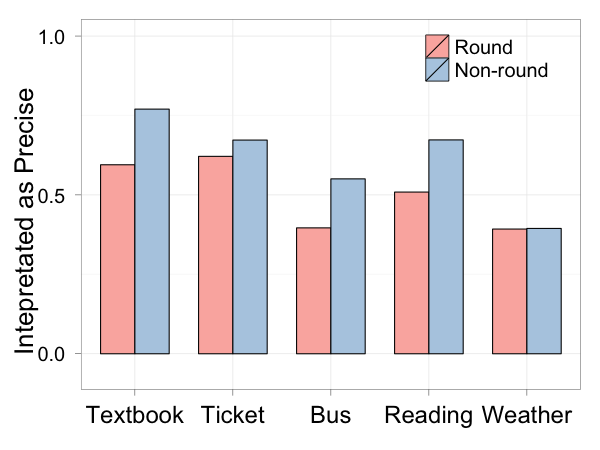
\includegraphics[width=\textwidth]{humans_halo_final.png}
		
	\end{subfigure} 
        \begin{subfigure}[b]{0.6\textwidth}
                \centering
                \caption{Exaggeration}
                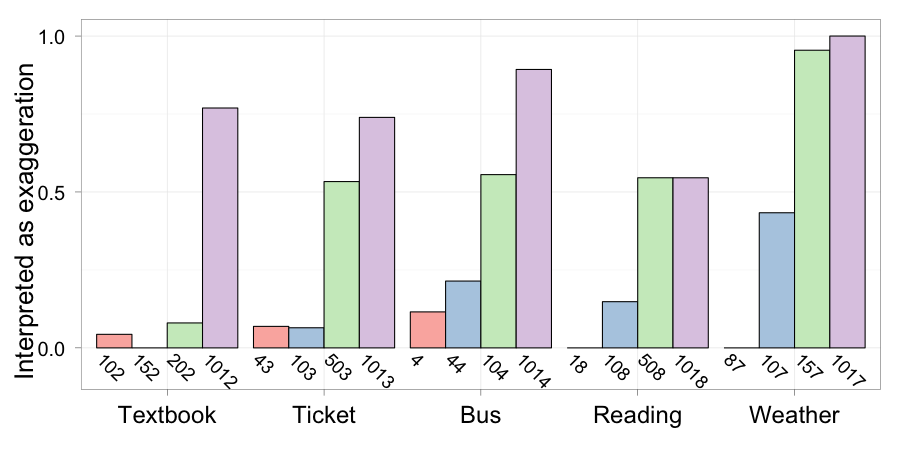
\includegraphics[width=\textwidth]{humans_exagg_all.png}
		
	\end{subfigure}
	\caption{Behavioral evidence for pragmatic halo and exaggeration effects across five scenarios}
\end{figure}

% Do we really want to discuss parking tickets here? We need to point readers to supplementary if we do.
Interestingly, the proportion of ``affect" responses varies across the five scenarios. In the parking ticket scenario, subjects are asked to judge how negatively a speaker who has just received a parking ticket feels about the ticket cost. Since the speaker is very likely to feel negatively about the ticket cost, the utterances are generally interpreted as having more negative affect than utterances in the textbook scenario. Our model can capture this effect by adjusting the prior probability of having an affective state regarding a particular scenario. 

\section{Discussion and Future Directions}


texttexttexttexttexttexttext texttexttexttexttexttextt exttexttexttexttexttexttextt exttexttexttexttexttexttexttextt exttext texttexttexttexttexttexttexttexttexttextt exttextt exttexttextte xttextt exttextt exttextte xttexttexttexttex ttexttexttextt exttextt exttexttextte xttextte xt texttexttexttextt exttextte xttexttexttextte xttexttexttextte xttext texttex ttexttex ttextte xttexttext texttexttextte xttexttexttext texttexttexttexttexttextt exttexttexttexttexttexttextt exttexttexttexttexttexttexttextt exttext texttexttexttexttexttexttexttexttexttextt exttextt exttexttextte xttextt exttextt exttextte xttexttexttexttex ttexttexttextt exttextt exttexttextte xttextte xt texttexttexttextt exttextte xttexttexttextte xttexttexttextte xttext texttex ttexttex ttextte xttexttext texttexttex ttexttexttextt exttexttexttexttexttexttextt exttexttexttexttexttexttexttextt exttext texttexttexttexttexttexttexttexttexttextt exttextt exttexttextte xttextt exttextt exttextte xttexttexttexttex ttexttexttextt exttextt exttexttextte xttextte xt texttexttexttextt exttextte xttexttexttextte xttexttexttextte xttext texttex ttexttex ttextte xttexttext texttexttexttexttexttexttext texttexttexttexttexttextt exttexttexttexttexttexttextt exttexttexttexttexttexttexttextt exttext texttexttexttexttexttexttexttexttexttextt exttextt exttexttextte xttextt exttextt exttextte xttexttexttexttex ttexttexttextt exttextt exttexttextte xttextte xt texttexttexttextt exttextte xttexttexttextte xttexttexttextte xttext texttex ttexttex ttextte xttexttext 
%\begin{figure}
%        \begin{subfigure}[b]{0.5\textwidth}
%                \centering
%		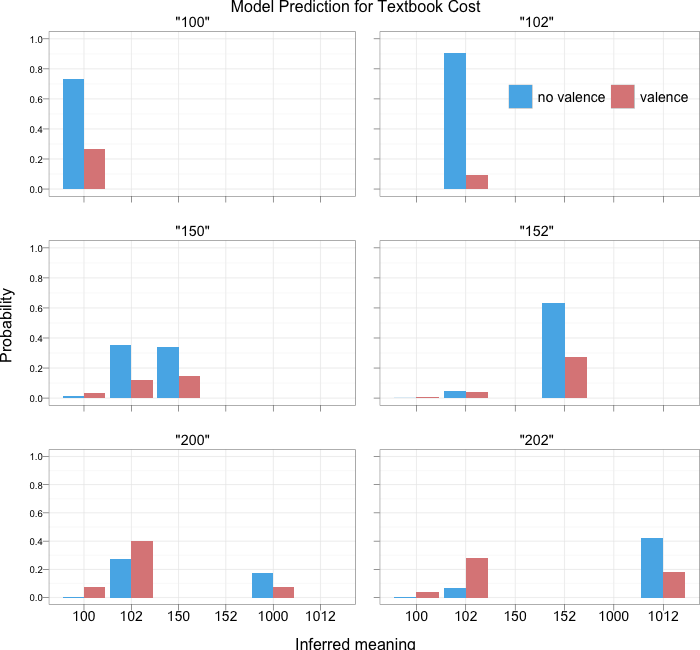
\includegraphics[width=\textwidth]{model_all_textbook.png}
%		\caption{model all textbook}
%	\end{subfigure}
%        \begin{subfigure}[b]{0.5\textwidth}
%                \centering
%                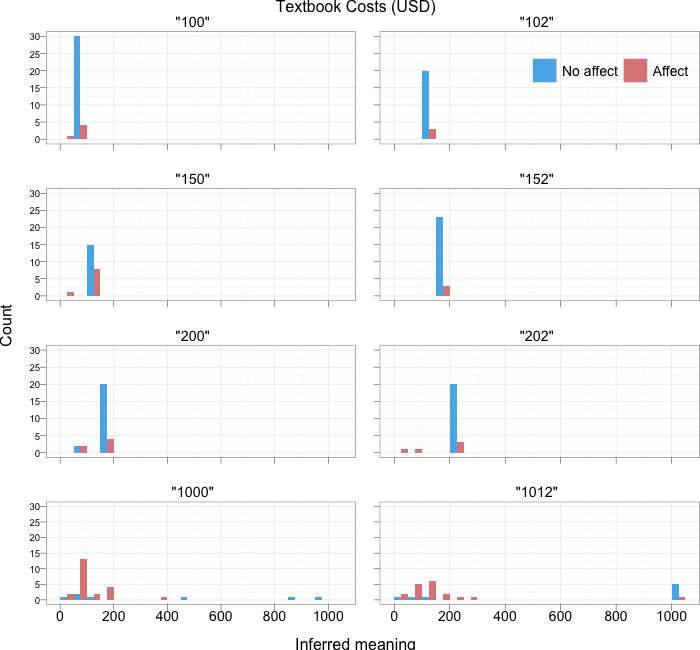
\includegraphics[width=\textwidth]{humans_all_textbook.png}
%		\caption{humans all textbook}
%	\end{subfigure}
%	\caption{The graph on the left shows rah rah rah and the one on the right shows roar roar roar}
%\end{figure}


\begin{figure}[t]
        \begin{subfigure}[b]{0.51\textwidth}
                \centering
                \caption{Model: Textbook costs}
                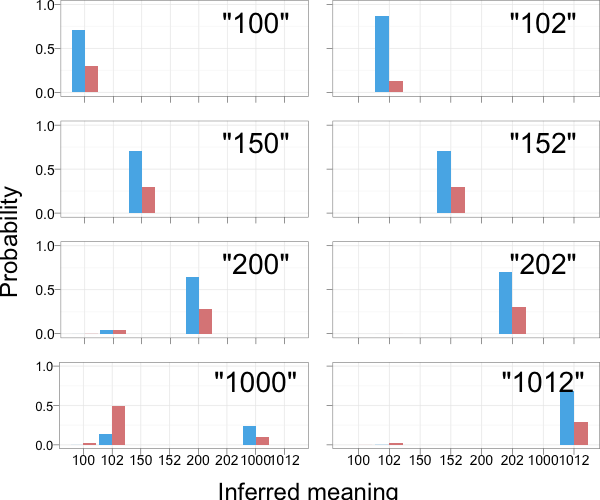
\includegraphics[width=\textwidth]{model_textbook_all.png}
	\end{subfigure}
        \begin{subfigure}[b]{0.51\textwidth}
                \centering
                \caption{Human: Textbook costs}
                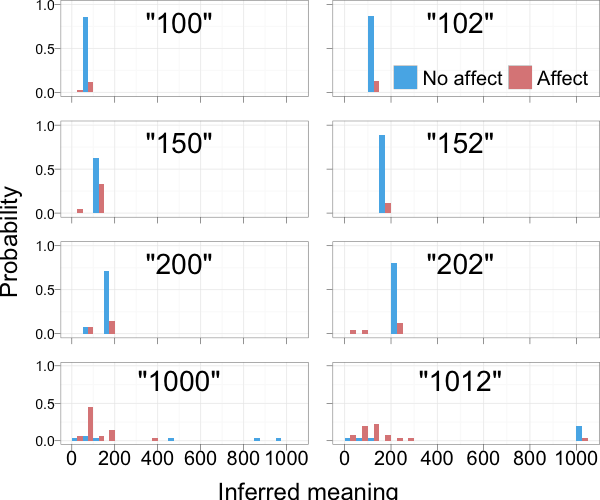
\includegraphics[width=\textwidth]{humans_textbook_all.png}
	\end{subfigure}
	\qquad
	
%\end{figure}
%\begin{figure}[t]
        \begin{subfigure}[b]{0.51\textwidth}
                \centering
                \caption{Model: Length of reading}
                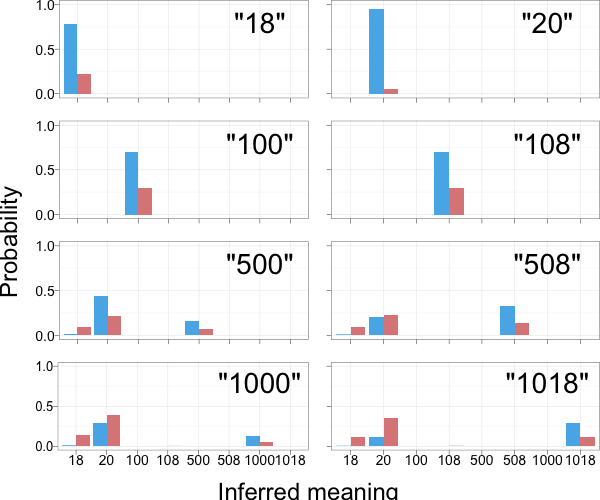
\includegraphics[width=\textwidth]{model_reading_all.png}
	\end{subfigure}
        \begin{subfigure}[b]{0.51\textwidth}
                \centering       
                \caption{Humans: Length of reading}         
                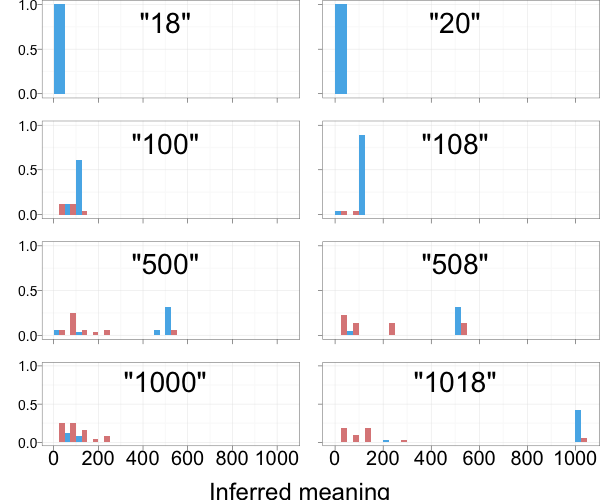
\includegraphics[width=\textwidth]{humans_reading_all.png}
        \end{subfigure}
        \qquad
        
%\end{figure}
%\begin{figure}[t]
        \begin{subfigure}[b]{0.51\textwidth}
                \centering
                \caption{Model: Weather temperature}
                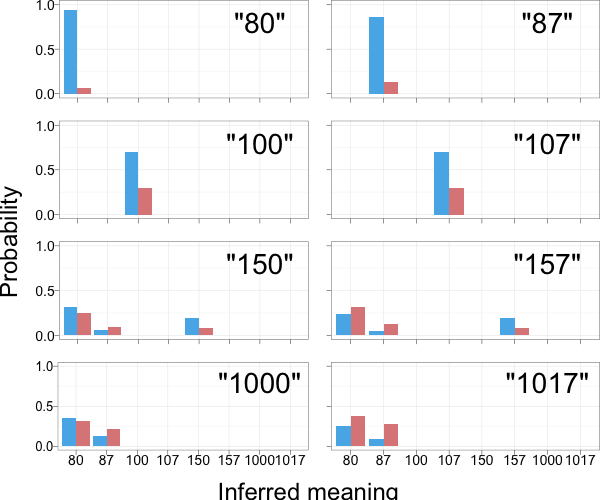
\includegraphics[width=\textwidth]{model_weather_all.png}
	\end{subfigure}
        \begin{subfigure}[b]{0.51\textwidth}
                \centering
                \caption{Humans: Weather temperature}
                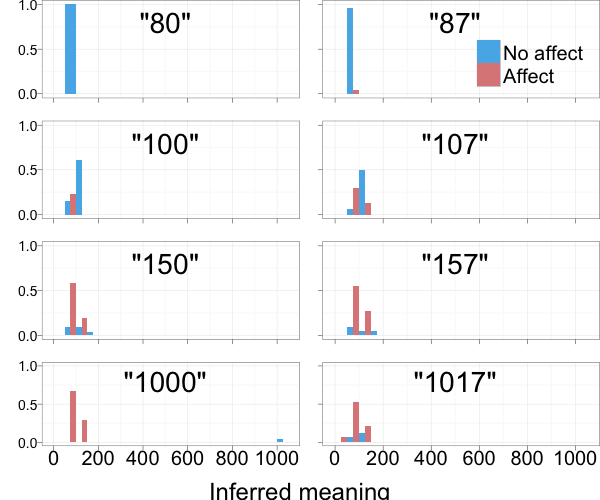
\includegraphics[width=\textwidth]{humans_weather_all.png}
        \end{subfigure}
	\caption{}
\end{figure}




\end{document}
